%%
%% 研究報告用スイッチ
%% [techrep]
%%
%% 欧文表記無しのスイッチ(etitle,jkeyword,eabstract,ekeywordは任意)
%% [noauthor]
%%

\documentclass[submit,techreq,noauthor,onecolumn]{ipsj}


\usepackage[dvipdfmx]{graphicx}
\usepackage{latexsym}

\def\Underline{\setbox0\hbox\bgroup\let\\\endUnderline}
\def\endUnderline{\vphantom{y}\egroup\smash{\underline{\box0}}\\}
\def\|{\verb|}

\setcounter{page}{1}

\pagestyle{empty}
\begin{document}


\title{Applied Type System}

\author{Hongwei Xi}{}{}

\begin{abstract}
Pure Type Systemフレームワーク ({\it PTS}) は型システムをデザイン/形式化する単純で一般的なアプローチを提供します。
けれども依存型の存在を認めると、一般帰納、再帰型、作用 (例: 例外、参照、入出力)、などのような多くの実際のプログラミングの機能に {\it PTS} を適用させることが難しくなります。
この論文では、実際のプログラミングの機能をサポートする型システムをたやすくデザイン/形式化できる、新しい Applied Type System ({\it ATS}) フレームワークを提案します。
{\it ATS} の鍵となる突出した機能は、コンストラクトされて評価されるプログラムを含む動的な部分から、形作られて根拠となる型を含む静的な部分を完全に分離することにあります。
この分離を用いると、{\it PTS} では許可されていましたが、プログラムが型の中に現われることは不可能になります。
{\it ATS} の形式的な開発だけでなく、実用的なプログラミングのための型システムを作るフレームワークとして {\it ATS} を使ったいくつかの例も紹介します。

この翻訳の元論文は http://www.ats-lang.org/PAPER/ATS-types03.pdf です。
\end{abstract}

\maketitle
\thispagestyle{empty}

\section{はじめに}
Pure Type Systemフレームワーク ({\it PTS}) [Bar92] は型システムをデザイン/形式化する単純で一般的なアプローチを提供します。
けれども依存型の存在を認めると、多くの実際のプログラミングの機能に {\it PTS} を適用させることが難しくなります。
とりわけ、一般帰納 [CS87]、再帰型 [Men87]、作用 [HMST95]、例外 [HN88]、入出力が存在するとき {\it PTS} を使って純粋性を担保するためには、多大な努力が必要になることを私達は学びました。
このような {\it PTS} の限界に対処するために、実際のプログラミングの機能をサポートする型システムをたやすくデザイン/形式化できる、新しい Applied Type System ({\it ATS}) フレームワークを提案します。
{\it ATS} の鍵となる突出した機能は、コンストラクトされて評価されるプログラムを含む動的な部分から、形作られて根拠となる型を含む静的な部分を完全に分離することにあります。
この分離は Dependent ML (DML) [XP99,Xi98] で開発された制限された依存型の成果に由来していて、参照や例外のような作用の存在下でも依存型を柔軟にサポートします。
また、{\it ガード型} ({\it guarded types}) と {\it アサート型} ({\it asserting types}) という2つの新しい (馴染みのない) 型を導入することで、{\it ATS} では {\it PTS} よりも柔軟に効果的にプログラムの不変条件を捕捉することができることを示します。

{\it ATS} のデザインと形式化がこの論文の主な主張で、[Zen97,XP99,XCC03] と似たアイデアを使った研究成果です。
{\it ATS} を使うと、{\it PTS} のある種生来の欠陥を乗り越えて、依存型の存在下で多くの一般的なプログラミングの機能をサポートする型システムをたやすく設計できます。
私達は現在 {\it ATS} に基づいた型システムを持ち、(DML で開発されたような) 依存型のみではなく guarded recursive datatypes [XCC03] をもサポートする、型付き関数型プログラミング言語を設計/実装している最中です。
Scheme が導入したようなアプローチ、つまり既存の言語に新しい言語構造を実装するような手法で、{\it ATS} を用いて多様な言語拡張をサポートできないか私達は探求しています。
とりわけ、オブジェクト指向プログラミング [XCC03]、メタプログラミング [XCC03,CX03]、型クラス [XCC02] のようないくつかのプログラミングの機能をこの手法で扱えることを、私達は既に示しています。

論文の残りは次のような構成になっています。
2章では、{\it ATS} フレームワークの詳細な開発成果を示します。
{\it ATS} で構成された汎用的な Applied Type System である ATS を形式化し、それから subject reduction と progress theorem を定義します。
3章では、{\it ATS} を拡張して、一般帰納、パターンマッチ、作用のような一般的で現実的なプログラミングの機能のいくつかに順応させます。
4章では、applied type system の興味深い例をいくつか示します。
最後に、関連研究と開発の将来の可能性について紹介した後、結論を述べます。
この論文はオンライン [Xi03] から入手できます。

\section{Applied Type System}

この章では Applied Type System ({\it ATS}) フレームワークの形式化を示します。
ここでは {\it ATS} で形式化された型システムを表わすのに {\it applied type system} という用語を使います。
この後の説明では、ATS を静的な要素 (statics) と動的な要素 (dynamics) から成る一般的な applied type system として定義します。
直感的に、statics と dynamics はそれぞれ型とプログラムを扱っています。
単純化のために、statics は簡単な純粋型付き言語であると仮定します。
そしてこの言語の型を {\it 種} ({\it sort}) という名前で呼ぶことにします。
statics の項を {\it 静的な項} ({\it static term}) と呼びます。
また dynamics の項を {\it 動的な項} ({\it dynamic term}) と呼びます。
そして、特別な種 {\it type} の静的な項は dynamics の型として機能します。

\begin{figure}[h]
\centering
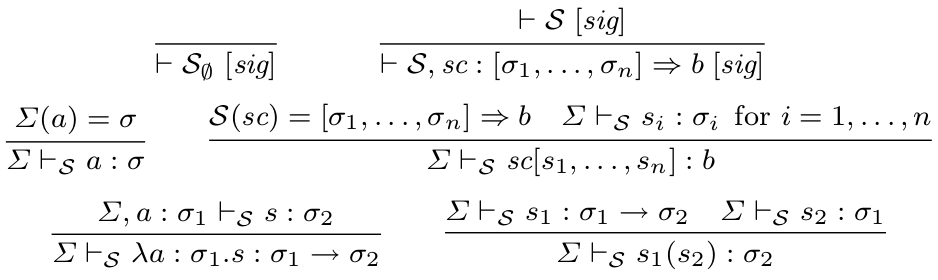
\includegraphics[width=14cm]{img/fig1_rules.png}
\caption{staticsを表わすシグニチャフォーマット規則と分類規則}
\label{fig:fig1_rules}
\end{figure}

\subsection{Statics}

静的な要素の形式的な表現を示します。
基礎種を表わすのに {\it b} と書きます。
2つの特別な基礎種 {\it type} と {\it bool} が存在すると仮定します。

\begin{figure}[h]
\centering
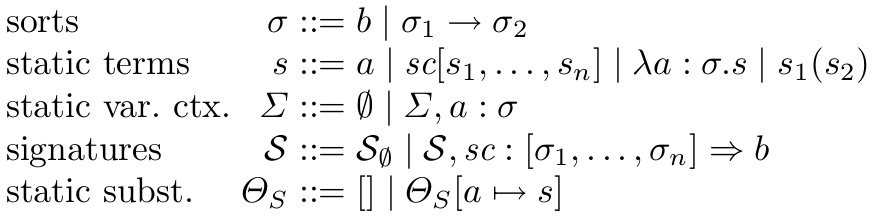
\includegraphics[width=12cm]{img/infig21_formaldesc.png}
\end{figure}

静的な項の変数は $\alpha$ を使って表わし、静的な項の集合を $s$ で表わします。
静的な定数 {\it sc} を宣言することもできます。
この定数は、静的な定数コンストラクタ {\it scc} もしくは静的な定数関数 {\it scf} のどちらかです。
sc種 (sc-sorts) を表わすのに [$\sigma_1$, $\ldots$ ,$\sigma_n$] $\Rightarrow$ {\it b} を使い、これは静的な定数に割り当てられます。
静的な定数 {\it sc} が与えられたとき、もし {\it sc} になんらかの種 $\sigma_1$, $\ldots$ ,$\sigma_n$ についてsc種 [$\sigma_1$, $\ldots$ ,$\sigma_n$] $\Rightarrow$ {\it b} が割り当てられていて、$i = 1, \ldots ,n$ について $s_i$ に種 $\sigma_i$ を割り当てることができるなら、種 {\it b} の項 {\it sc}[$s_1$, $\ldots$ ,$s_n$] を作ることができます。
誤解を生じない場合は、{\it sc}[] を {\it sc} と書くことができます。
sc種は (標準の) 種とは見なされていないことに注意してください。

xxx

\begin{figure}[h]
\centering
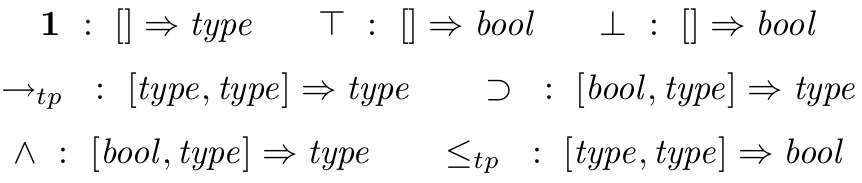
\includegraphics[width=12cm]{img/infig21_initialsig.png}
\end{figure}



\begin{acknowledgment}
\end{acknowledgment}

\begin{thebibliography}{10}
\end{thebibliography}

\end{document}
